\icode{N16H-MD-SI-L2-261111-002}
\nceeID[2]{2016上海}{4}
如图所示，顶端固定着小球的直杆固定在小车上，当小车向右做匀加速运动时，球所受合外力的方向沿图中的\paren[]
	
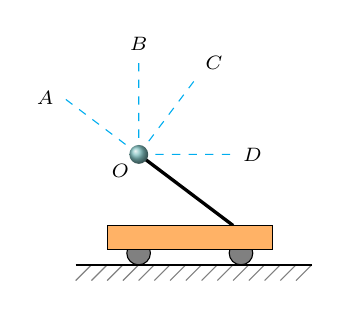
\begin{tikzpicture}[font=\scriptsize]
	\draw[very thick] (0,0)--(143:1.5)coordinate(o);
	\draw[dashed,cyan] (o)node[below left,black]{\(O\)}--++(143:1.2)node[left,black]{\(A\)} (o)--++(90:1.2)node[above,black]{\(B\)} (o)--++(53:1.2)node[above right,black]{\(C\)} (o)--++(0:1.2)node[right,black]{\(D\)};
	\shade[ball color=teal!50] (o) circle(.12);
	\draw[fill=gray] (-1.2,-.35) circle(.15) (.1,-.35) circle(.15);
	\draw[fill=orange!60] (-1.6,0) rectangle(.5,-.3);
	\foreach \x in {-2,-1.8,...,.8}
		\draw[gray] (\x,-.7)--++(.2,.2);
	\draw[thick] (-2,-.5)--(1,-.5);
\end{tikzpicture}
\begin{choices}
	\item \(OA\) 方向
	\item \(OB\) 方向
	\item \(OC\) 方向
	\item \(OD\) 方向
\end{choices}
\begin{answer}
	C\quad 提示：小车向右{\color{red}匀加速}运动，可知小球合外力向右
\end{answer}